\documentclass[tikz,convert={density=800,outext=.png},border=5pt]{standalone}
%\documentclass[preview]{standalone}

\usepackage[utf8]{inputenc}					% Выбор языка и кодировки
\usepackage{amsmath} % nice math symbols
     
\usepackage{tikz}
\usetikzlibrary{shapes,positioning,calc}

\newcommand{\opredictors}[4]{
	\node[z_pred, minimum width = #2pt, minimum height = #2pt] (z_#1) at ($(#3,#4)$) {};
	\node[z_pred, minimum width = #2, minimum height = #2] at ($(z_#1)+(#2/500.0,-#2/1000.0)$) {};
	\node[z_pred, minimum width = #2, minimum height = #2] at ($(z_#1)+(#2*2/500.0,-#2*2/1000.0)$) {};
	\node (point_#1) at ($(z_#1)+(0,-#2/500)$) {$\cdot$};			
	\node at ($(point_#1)+(#2/1500.0,-#2/1500.0)$) {$\cdot$};
	\node at ($(point_#1)+(#2/750.0,-#2/750.0)$) {$\cdot$};
	\node[z_pred, minimum width = #2, minimum height = #2] (z_l_#1) at ($(z_#1)+(#2/125.0,-#2/250.0)$) {};
	
	\draw[ultra thick, gray!60!black] ($(z_l_#1)+(-3pt,4.5pt)$) -- ($(z_l_#1)+(-3pt,-4.5pt)$);
	\node at (z_l_#1) {$\cdots$};
	\node[font=\small] at ($(z_l_#1)+(-1pt,-3pt)$) { $z_1$};
	\node[font=\small] at ($(z_l_#1)+(1pt,3pt)$) {$z_h$};
	\draw[ultra thick, gray!60!black] ($(z_l_#1)+(3pt,4.5pt)$) -- ($(z_l_#1)+(3pt,-4.5pt)$);
}	

\newcommand{\ppredictors}[4]{
	\node[z_pred, minimum width = #2pt, minimum height = #2pt] (z_#1) at ($(#3,#4)$) {};
	\node[z_pred, minimum width = #2, minimum height = #2] at ($(z_#1)+(#2/500.0,-#2/1000.0)$) {};
	\node[z_pred, minimum width = #2, minimum height = #2] at ($(z_#1)+(#2*2/500.0,-#2*2/1000.0)$) {};
	\node (point_#1) at ($(z_#1)+(0,-#2/500)$) {$\cdot$};			
	\node at ($(point_#1)+(#2/1500.0,-#2/1500.0)$) {$\cdot$};
	\node at ($(point_#1)+(#2/750.0,-#2/750.0)$) {$\cdot$};
	\node[z_pred, minimum width = #2, minimum height = #2] (z_l_#1) at ($(z_#1)+(#2/125.0,-#2/250.0)$) {};
	
	\draw[ultra thick, gray!60!black] ($(z_l_#1)+(-3pt,4.5pt)$) -- ($(z_l_#1)+(-3pt,-4.5pt)$);
	\draw[->] ($(z_l_#1)+(-2.5pt,0)$) to[out=50,in=210] ($(z_l_#1)+(2.5pt,0)$);
	\node[font=\small] at ($(z_l_#1)+(-1pt,-3pt)$) {$z^c$};
	\node[font=\small] at ($(z_l_#1)+(1pt,3pt)$) {$z^e$};
	\draw[ultra thick, gray!60!black] ($(z_l_#1)+(3pt,4.5pt)$) -- ($(z_l_#1)+(3pt,-4.5pt)$);
}	

\begin{document}
	
	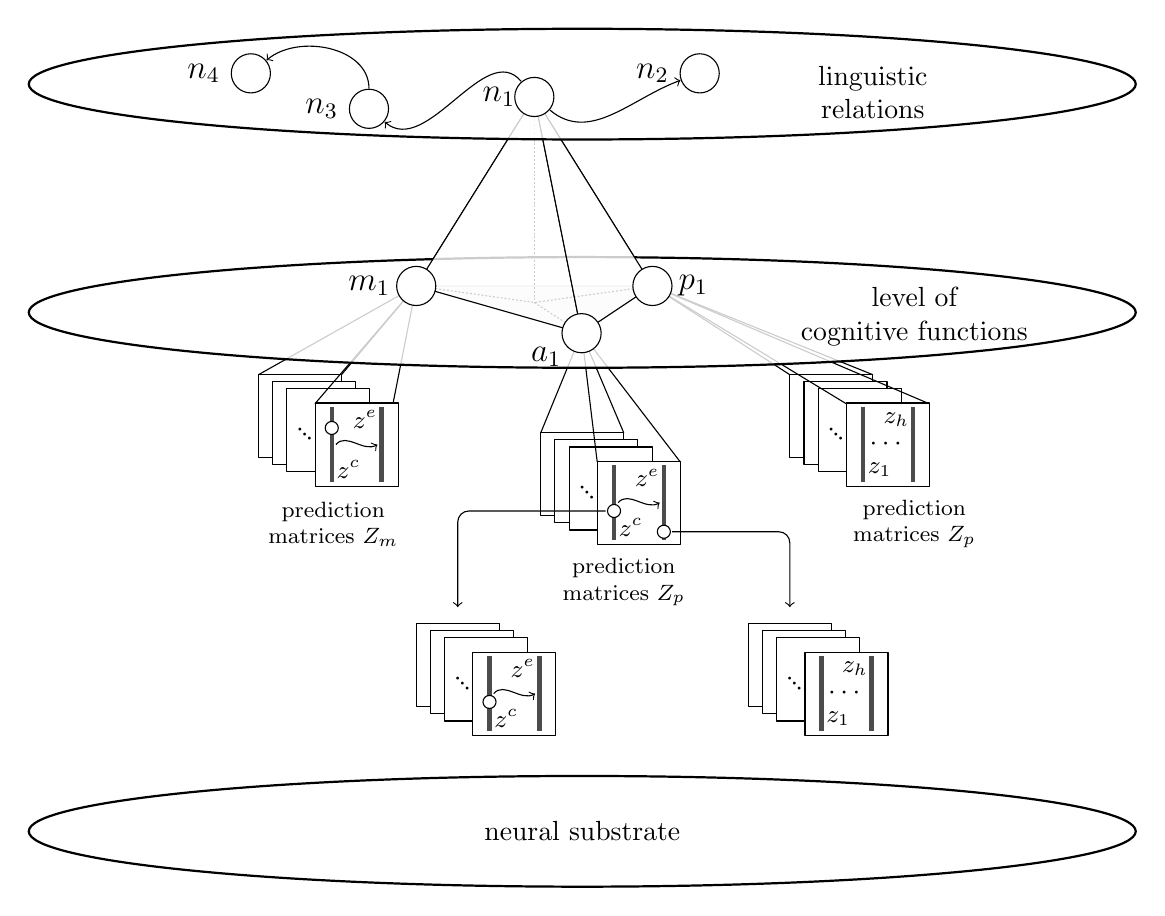
\begin{tikzpicture}[join=round,scale=3.0,node distance = -0.05]
		\tikzstyle{sign_comp}=[draw, circle,fill=white, scale=1.5];
		\tikzstyle{label_small}=[align=center,font=\footnotesize,fill=white,opacity=0.8,text opacity=1];
		\tikzstyle{coord_cine}=[dash pattern=on 0.7 off 0.7];
		
		\tikzstyle{z_pred}=[draw, rectangle,fill=white];


		\filldraw[fill=white] (0.0,0.2) -- (0.5,1.0) -- (1.0,0.2) -- cycle;
		\filldraw[fill=black!20] (0.0,0.2) -- (0.7,0.0) -- (1.0,0.2) -- cycle;
		
	
		\node (s_m) at (0.0,0.2) {};
		\node (s_p) at (1.0,0.2) {};
		\node (s_a) at (0.7,0.0) {};

		\ppredictors{m}{30}{-14pt}{-10pt}		
		\draw[thin] (-9pt,-5pt) -- (s_m);
		\draw[thin] (-19pt,-5pt) -- (s_m);
		\draw[thin] (-2.8pt,-8.5pt)  -- (s_m);
		\draw[thin] (-12.2pt,-8.5pt) -- (s_m);
		\node[align=center,font=\footnotesize] at (-10pt,-23pt) {prediction\\matrices $Z_m$};		
		
		\opredictors{p}{30}{50pt}{-10pt}		
		\draw[thin] (55pt,-5pt) -- (s_p);
		\draw[thin] (45pt,-5pt) -- (s_p);
		\draw[thin] (61.8pt,-8.5pt)  -- (s_p);
		\draw[thin] (51.8pt,-8.5pt) -- (s_p);
		\node[align=center,font=\footnotesize] at (60pt,-23pt) {prediction\\matrices $Z_p$};
		

		\ppredictors{a}{30}{20pt}{-17pt}	
		\draw[thin] (25pt,-12pt) -- (s_a);
		\draw[thin] (15pt,-12pt) -- (s_a);
		\draw[thin] (31.8pt,-15.5pt)  -- (s_a);
		\draw[thin] (21.8pt,-15.5pt) -- (s_a);	
		\node[align=center,font=\footnotesize] at (25pt,-30pt) {prediction\\matrices $Z_p$};

		\node[draw, thick, ellipse, fill=white, fill opacity=0.8, minimum width=400, minimum height = 40] at (20pt,2.5pt){};
		\draw[coord_cine] (0.5,1.0) -- (0.5,0.13);
		\draw[coord_cine] (0.0,0.2) -- (0.5,0.13);
		\draw[coord_cine] (0.7,0.0) -- (0.5,0.13);
		\draw[coord_cine] (1.0,0.2) -- (0.5,0.13);
		\filldraw[fill=white,fill opacity=0.8] (0.0,0.2) -- (0.5,1.0) -- (0.7,0.0) -- cycle;
		\filldraw[fill=white,fill opacity=0.8] (0.7,0.0) -- (0.5,1.0) -- (1.0,0.2) -- cycle;

		\node[draw, thick, ellipse, fill=white, fill opacity=0.8, minimum width=400, minimum height = 40] at (20pt,30pt){};
		\node[align=center] at (55pt,29pt) {linguistic\\relations};
		\node[align=center] at (60pt,2pt) {level of\\cognitive functions};

		\node[sign_comp] (s_m) at (0.0,0.2) {};
		\node[sign_comp] (s_p) at (1.0,0.2) {};
		\node[sign_comp] (s_a) at (0.7,0.0) {};
		\node[sign_comp] (s_n) at (0.5,1.0) {};		
		\node[sign_comp] (s_n2) at (1.2,1.1) {};

		\node[align=center, font=\large] at ($(s_n2)+(-0.20,-0.0)$) {$n_2$};
		\node[sign_comp] (s_n3) at (-0.2,0.95) {};
		\node[align=center, font=\large] at ($(s_n3)+(-0.20,-0.0)$) {$n_3$};
		\node[sign_comp] (s_n4) at (-0.7,1.1) {};
		\node[align=center, font=\large] at ($(s_n4)+(-0.20,-0.0)$) {$n_4$};
		\node[align=center, font=\large] at ($(s_n)+(-0.15,-0.0)$) {$n_1$};
		\draw[->,rounded corners] (s_n) to[out=-40,in=200] (s_n2);
		\draw[->,rounded corners] (s_n) to[out=130,in=-40] (s_n3);
		\draw[->,rounded corners] (s_n3) to[out=90,in=40] (s_n4);


		\node[left = of s_m, font=\large] {$m_1$};
		\node[right = of s_p, font=\large]{$p_1$};
		\node[align=center, font=\large] at ($(s_a)+(-0.15,-0.1)$) {$a_1$};		
		

		\opredictors{a1}{30}{45pt}{-40pt}
		
		\ppredictors{a2}{30}{5pt}{-40pt}
		\draw[->,rounded corners] ($(z_l_a)+(-4pt,-1pt)$) -- ($(z_l_a)+(-10pt,-1pt)$) -| ($(z_a2)+(0,7pt)$);
		\node[draw, circle, fill=white, scale=0.5] at ($(z_l_a)+(-3pt,-1pt)$) {};
		\draw[->,rounded corners] ($(z_l_a)+(4pt,-3.5pt)$) -- ($(z_l_a)+(10pt,-3.5pt)$) -| ($(z_a1)+(0,7pt)$);
		\node[draw, circle, fill=white, scale=0.5] at ($(z_l_a)+(3pt,-3.5pt)$) {};
		
		\node[draw, circle, fill=white, scale=0.5] at ($(z_l_a2)+(-3pt,-1pt)$) {};
		\node[draw, circle, fill=white, scale=0.5] at ($(z_l_m)+(-3pt,2pt)$) {};

		\node[draw, thick, ellipse, fill=white, fill opacity=0.8, minimum width=400, minimum height = 40] at (20pt,-60pt){};
		\node[align=center] at (20pt,-60pt) {neural substrate};
	\end{tikzpicture}


\end{document}